% IEEE-style draft. IEEEtran is used when installed; portable fallback is explicit.
\IfFileExists{IEEEtran.cls}{\documentclass[conference]{IEEEtran}}{\documentclass[10pt,twocolumn]{article}\usepackage[margin=0.75in]{geometry}}
\usepackage{graphicx,amsmath,array,url}
\newcommand{\pending}{\textit{Not evaluated}}
\title{Robust Detection of AI-Generated Speech Across Unseen Voice Synthesis Models Using Deep Learning and Hybrid Acoustic Representations}
\author{Author names, affiliations and contributions pending}
\date{}
\begin{document}
\maketitle
\begin{abstract}
VoxGuard AI is a reproducible research system for genuine pretrained audio anti-spoofing inference. Bounded decoding and versioned model loading produce uncalibrated scores; a reviewed, domain-specific validation policy is required before human/synthetic decisions are enabled. The experimental protocol separates speakers, original recordings and synthesis families, and distinguishes prediction abstention from binary error metrics. A six-recording English convenience pilot confirms actual inference on licensed human speech and locally generated classical synthesis. The same six recordings yield 36 paired clean, noise and codec observations. These observations are not representative benchmark evidence: modern neural synthesis, unseen generators, multilingual performance, threshold validation and hybrid improvements remain unestablished. This draft presents implementation and falsifiable research methodology rather than a claim of detector reliability or algorithmic novelty.
\end{abstract}
\noindent\textbf{Draft status:} Research protocol and measured engineering pilot. Not submission-ready. Venue formatting, authorship and representative empirical results remain pending.

\section{Introduction}
Synthetic speech may imitate plausible human recordings, but authentic speech can also trigger detector errors. Practical analysis therefore requires reproducible provenance, conservative interpretation and independent evaluation. We study whether frozen learned speech representations and frequency-domain features improve held-out-generator discrimination relative to a verified anti-spoofing baseline. A model score does not prove authenticity, identify a synthesis platform or establish speaker identity.

\section{Related Work}
AASIST combines spectro-temporal graph attention for anti-spoofing\cite{jung2021aasist}; RawNet2 is an established end-to-end baseline\cite{tak2021rawnet2}. ASVspoof 2019 defines standardized evaluation material and protocols\cite{wang2020asvspoof}. Wav2vec 2.0 learns speech representations through self-supervision\cite{baevski2020wav2vec}, but an encoder is not by itself a spoof detector. WaveFake supplies a generated-audio dataset and experimental context\cite{frank2021wavefake}. Published baseline metrics are not copied into our result table because dataset, operating point and protocol equivalence have not been established.

\section{Research Gap}
Synthesis-family, channel and language shifts can invalidate conclusions based on familiar generators. Repeated source utterances and shared speakers can create leakage; codec differences can create shortcuts. These established concerns motivate project-specific generator-held-out and source-disjoint testing. Their investigation is a hypothesis, not an assertion of novelty.

\section{Problem Formulation}
For recording $x$, preprocessing $P$ produces mono 16 kHz samples, and frozen detector $f$ produces a synthetic-oriented score $s=f(P(x))\in[0,1]$. The score is uncalibrated and is not a probability of authenticity. A validation-derived policy with $t_h<t_a$ returns
\begin{equation}
\hat y=\begin{cases}\mathrm{human},&s\le t_h,\\\mathrm{synthetic},&s\ge t_a,\\\mathrm{uncertain},&\text{otherwise}.\end{cases}
\end{equation}
Without a reviewed policy, every recording abstains. Synthetic speech is the positive class. Coverage and per-class abstention must accompany accepted-only accuracy; abstentions must not silently disappear from error denominators.

\section{Methodology}
The established baseline is the official frozen AASIST checkpoint. Proposed comparisons use frozen speech embeddings, LFCC summaries and a small fusion head. Normalization uses training data only; validation selects checkpoints and operating thresholds; untouched test data estimates final performance. Generator-held-out studies exclude test synthesis families from both training and validation. All encodings, crops and augmentations remain with their original source split. Unknown overlap with representation pretraining is disclosed.

\section{Model Architecture}
The baseline is vendored unchanged from the NAVER AASIST repository, source revision \texttt{a04c9863f63d44471dde8a6abcb3b082b07cd1d1}. The strict weights-only checkpoint is verified by SHA-256, recorded in the accompanying result artifacts. Upstream label 0 is spoof and label 1 bona fide. Input windows contain 64,600 samples; short inputs repeat-pad according to upstream preprocessing. Long recordings use contiguous windows and a duration-weighted mean of spoof-class softmax outputs. This aggregation is an application extension requiring validation. Window scores are not exact edit localization. No voice-activity detector is applied.

The research-only encoder is official TorchAudio WAV2VEC2\_BASE. Final-layer temporal mean and population standard deviation provide 1,536 learned dimensions; LFCC mean/standard deviation add 40 dimensions. Four-second windows bound attention memory. A separate 64-unit fusion head supports learned-only, acoustic-only and hybrid ablations; no trained production hybrid or demonstrated improvement is supplied.

\section{Dataset Description}
The engineering pilot contains three original LibriSpeech excerpts with individually inspected CC-BY-4.0 attribution and three local Flite recordings using project-authored text. Flite is classical, non-neural synthesis, not modern voice cloning. The six recordings are test-only; no training or validation split is inferred. Human and synthetic recording domains differ, making shortcut explanations plausible. Unknown overlap with pretraining cannot be ruled out. Source URLs, checksums, attribution and generation commands are retained in dataset documentation and provenance artifacts. User uploads are never added to training automatically.

Target representative corpora include ASVspoof 2019 LA, ASVspoof 5, WaveFake and authorized in-the-wild recordings, subject to inspected rights, official protocols and availability. A subsequent access audit found official ASVspoof tools and WaveFake software reachable through GitHub, but tool/fixture code licenses did not establish recording rights or evaluation coverage. Authoritative recording/rights hosts remained blocked by the network proxy; no bypass was attempted. No new representative validation or test corpus was acquired. A reproducible engineering rerun reused the same six pilot recordings and explicitly reported zero validation rows and an unestablished policy; it is not additional independent evidence. Hindi/Marathi studies require licensed or consented, provenance-labeled human and synthetic examples; English results establish no Indic-language capability.

\section{Experimental Setup}
Decoding uses FFmpeg mono float samples at 16 kHz. The API bounds upload size and duration; the research decoder's 120-second cap must be disclosed or avoided through a documented segmentation policy. Record checkpoint, score-protocol, manifest and score digests, Git revision, software versions, hardware, thread count and random seeds. The observed pilot used Python 3.12.14, PyTorch 2.6 CPU, NumPy 1.26.4 and two inference threads.

Primary metrics are AUROC and interpolated EER; fixed-threshold metrics include precision, recall, F1, accuracy, FPR, FNR and confusion matrices. A separate two-threshold report includes coverage and abstentions. Validation fitting and test scoring verify model/protocol provenance and identity separation. Speaker-cluster bootstrap intervals are appropriate when sampling assumptions and sample counts support them. The tiny pilot does not support population-level confidence claims.

\section{Results and Discussion}
Table~\ref{tab:pilot} reports descriptive measurements only. All six convenience examples are rank-separated by the baseline; there is no validated operating threshold, binary accuracy or modern-generator claim. The 36 observations reuse six source recordings and are not 36 independent samples.
\begin{table}[t]\centering\small
\caption{Tiny convenience pilot: 3 human and 3 classical Flite recordings. Descriptive ranking, not representative reliability.}\label{tab:pilot}
\begin{tabular}{lrrr}\hline
Condition & Sources & AUROC & EER\\\hline
Clean & 6 & 1.0 & 0.0\\
White noise 20 dB & 6 & 1.0 & 0.0\\
White noise 10 dB & 6 & 1.0 & 0.0\\
MP3 32 kbps & 6 & 1.0 & 0.0\\
MP3 64 kbps & 6 & 1.0 & 0.0\\
AAC 64 kbps & 6 & 1.0 & 0.0\\\hline
\end{tabular}
\end{table}
\IfFileExists{pilot_scores.pdf}{\begin{figure}[t]\centering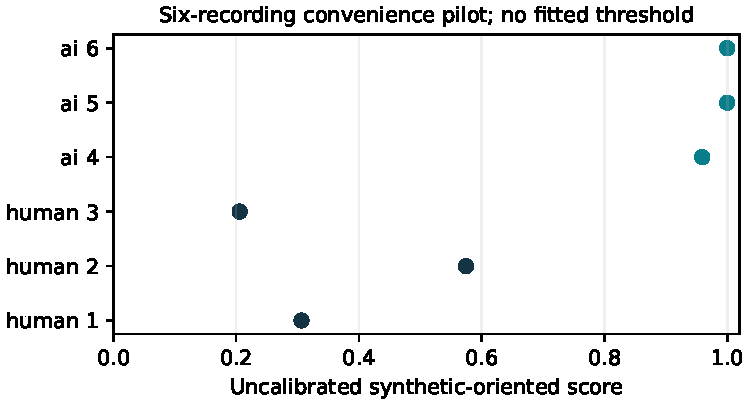
\includegraphics[width=\columnwidth]{pilot_scores.pdf}\caption{Actual clean scores for the six convenience recordings. No decision boundary is fitted. Rank separation here does not establish population accuracy.}\end{figure}}{}
A separate 4.39-second synthetic-speech run measured 573.55 ms cold and 460.26 ms warm inference, excluding decoding. Peak process RSS was 495,194,112 bytes including interpreter/imports. These are hardware- and run-specific observations, not Windows performance or service-throughput guarantees.

\begin{table}[t]\centering\small
\caption{Required representative comparisons. No missing experiment is replaced with a pilot result.}
\begin{tabular}{p{.48\columnwidth}p{.39\columnwidth}}\hline
Experiment & Status\\\hline
Official held-out baseline & \pending\\
Modern/unseen synthesis families & \pending\\
Hindi / Marathi & \pending\\
Hybrid versus matched baselines & \pending\\
Independent threshold test & \pending\\\hline
\end{tabular}
\end{table}

\section{Ablation Study}
Use identical identity-audited partitions and at least three fixed seeds for learned-only, LFCC-only and fusion heads. Compare augmentation off/on with paired clean, noise, MP3 and AAC material. Match hyperparameter-search budgets and report parameter count, cost and failure cases. These experiments remain pending suitable labeled data. Extracting genuine pretrained features is not evidence of hybrid classification performance.

\section{Limitations}
The old English-centric checkpoint is not validated for modern generators, adversarial edits, Hindi or Marathi. Silence, music and out-of-domain signals may produce misleading outputs. Default abstention is a deliberate consequence of missing validation evidence. The pilot has tiny counts, domain confounding and possible pretraining overlap. No universal accuracy, novelty, calibrated probability or exact manipulation-localization claim is made. External datasets may require license review, authorization or network access not available here. Failed acquisition attempts are recorded rather than silently substituted. Public deployment and full Windows/CUDA execution are separate from local Linux evidence.

\section{Conclusion}
VoxGuard AI provides genuine, provenance-checked inference and reproducible evaluation infrastructure. The measured convenience pilot verifies software behavior and a narrow ranking observation, not detector reliability. Representative validation and untouched test corpora, language/generator-held-out studies and controlled hybrid ablations remain prerequisites to empirical conclusions or submission readiness.

\IfFileExists{IEEEtran.bst}{\bibliographystyle{IEEEtran}}{\bibliographystyle{unsrt}}
\bibliography{references}
\end{document}
